\documentclass[a4paper,12pt]{article}

%%% Работа с русским языком
\usepackage{cmap}					% поиск в PDF
\usepackage{mathtext} 				% русские буквы в фомулах
\usepackage[T2A]{fontenc}			% кодировка
\usepackage[utf8]{inputenc}			% кодировка исходного текста
\usepackage[english,russian]{babel}	% локализация и переносы
\usepackage[left=25mm, top=15mm, right=20mm, bottom=15mm, nohead, footskip=10mm]{geometry}
%%% Дополнительная работа с математикой
\usepackage{amsfonts,amssymb,amsthm,mathtools} % AMS
\usepackage{amsmath}
\usepackage{icomma} % "Умная" запятая: $0,2$ --- число, $0, 2$ --- перечисление

%% Номера формул
%\mathtoolsset{showonlyrefs=true} % Показывать номера только у тех формул, на которые есть \eqref{} в тексте.

%% Шрифты
\usepackage{euscript}	 % Шрифт Евклид
\usepackage{mathrsfs} % Красивый матшрифт

%% Свои команды
\DeclareMathOperator{\sgn}{\mathop{sgn}}

%% Перенос знаков в формулах (по Львовскому)
\newcommand*{\hm}[1]{#1\nobreak\discretionary{}
{\hbox{$\mathsurround=0pt #1$}}{}}

%%% Работа с картинками
\usepackage{graphicx}  % Для вставки рисунков
\graphicspath{{images/}{images2/}}  % папки с картинками
\setlength\fboxsep{3pt} % Отступ рамки \fbox{} от рисунка
\setlength\fboxrule{1pt} % Толщина линий рамки \fbox{}
\usepackage{wrapfig} % Обтекание рисунков и таблиц текстом

%%% Работа с таблицами
\usepackage{array,tabularx,tabulary,booktabs} % Дополнительная работа с таблицами
\usepackage{longtable}  % Длинные таблицы
\usepackage{multirow} % Слияние строк в таблице
%%% Ссылки внутри документа
\usepackage[unicode, pdftex]{hyperref}
%%% Заголовок
\usepackage{graphicx}
\usepackage{wrapfig}
\usepackage{listings}
\usepackage{color}

\definecolor{dkgreen}{rgb}{0,0.6,0}
\definecolor{gray}{rgb}{0.5,0.5,0.5}
\definecolor{mauve}{rgb}{0.58,0,0.82}


\begin{document} 
% Set default path for images
\graphicspath{ {./imgs/} }
\title{Заметки о системах линейных уравнений}
\author{https://github.com/enlacroix}
\maketitle

\begin{center}
    \textsc{Системы линейных уравнений I: \\
    Визуализация. Теорема Фредгольма}
\end{center}
\begin{center}
    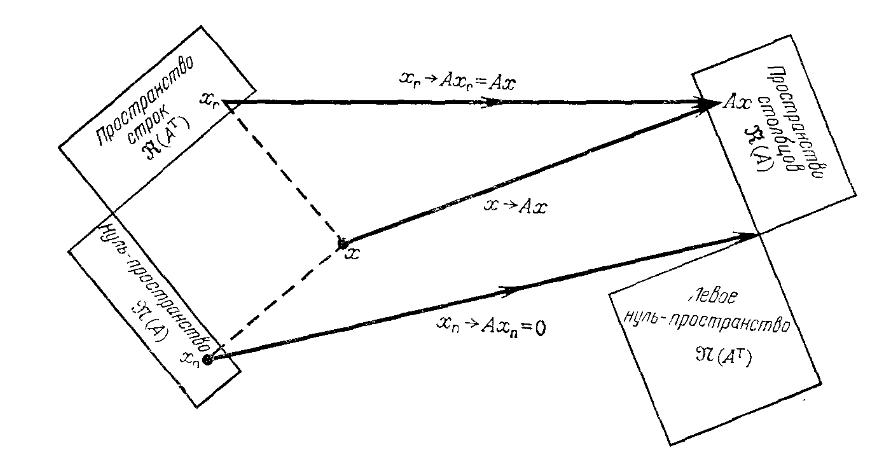
\includegraphics[width = 13.5 cm]{bigpict.PNG}
\end{center}
\begin{center}
    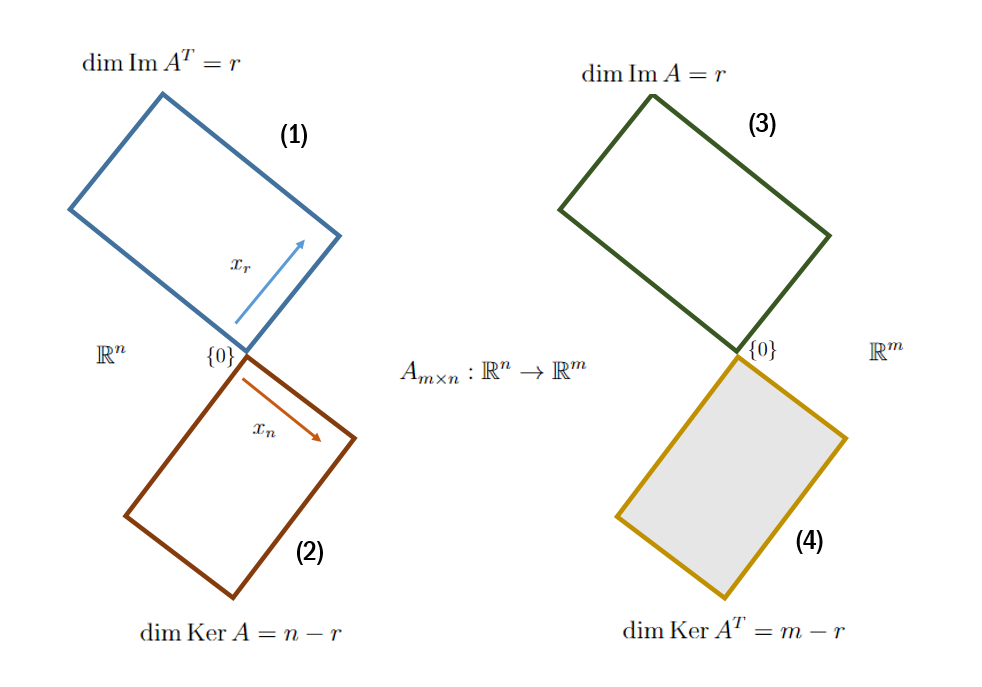
\includegraphics[width = 15 cm]{fff.PNG}
\end{center}
\newpage
Приведенные выше рисунки называют также '\textit{big picture of linear algebra}'. Сверху представлена версия с терминологией, принятой в западном изложении линейной алгебры, снизу - с привычными нам понятиями образа и ядра. \\
Суть в том, что систему линейных уравнений в матричной форме $Ax = b$ можно представить, как действие линейного преобразования $A$ на произвольный вектор $x$. $A$ описывается четырьмя подпространствами: пространством строк, пространством столбцов, нуль-пространством и левым нуль-пространством. \\
Например, \textit{пространство строк} - всевозможные линейные комбинации строк матрицы $A$. Вектор $x$ раскладывается на две составляющие $x_r \in Im A^T$, проекция на пространство строк, и $x_n \in Ker A$ - ортогональная составляющая. Компонента $x_n$ это ядро преобразования, решение системы $Af =0$. $A$ переводит $x_n$ в левое нуль-пространство ($Ker A^T$). Вторая компонента $x_r$ раскладывается по строкам матрицы $A$ и $Ax_r = b \in Im A$. \\
Данный подход полезен своей наглядностью. \textbf{Теорема Кронекера-Капелли}, которая гарантирует совместность системы при равенстве ранга основной и расширенной (добавили к основной столбец $b$) матрицы. Следовательно, $b \in \operatorname{Im} A$, иными словами принадлежит \textit{пространству столбцов} - существует линейная комбинация, через которую выразится правая часть. Подпространства (1) и (2), (3) и (4) пересекаются только в нулевом векторе. Отметим, что:
\[ \operatorname{Im} A^{T} \perp \operatorname{Ker} A  \]
\[ \operatorname{Ker} A^{T} \perp \operatorname{Im} A \]
Пространство $\mathbb{R}^m$ раскладывается на прямую сумму подпространств (3) и (4). Аналогично $\mathbb{R}^n = \operatorname{Im} A^{T} \oplus \operatorname{Ker} A$. \\
Можно придумать одно упражнение, основанное на этом факте: \\
\textit{
Решить систему уравнений 
\begin{equation*}
 \begin{cases}
   x + 2y + 3z = 0\\
   4x + 5y + 6z = 0
 \end{cases}
\end{equation*}
Не используйте метод Гаусса или любой другой известный вам классический способ решения (в том числе и школьные). } \\
Разгадка состоит в том, что искомый вектор ортогонален пространству строк. Так как мы работаем в трехмерном пространстве, то можно воспользоваться векторным произведением для нахождения столбца фундаметальной системы решений. \\
Подчеркнём, что $b \perp \forall w \in  \operatorname{Ker} A^{T}$, в силу ортогональности подпространств. Вектора, лежащие в подпространстве (4) описываются системой уравнений:
\[ A^T w = 0\]
Это ни что иное, как \textbf{теорема Фредгольма}. Напомним ее: \\
\textbf{Теорема Фредгольма о системах линейных уравнений.}\\
Для того чтобы система $Ax = b$ была совместна, \textit{необходимо и достаточно}, чтобы каждое решение сопряженной однородной системы $A^Tw = 0$ удовлетворяло уравнению $w^Tb = 0$. \\
Наглядное представление позволяет с легкостью восстановить классическое доказательство данной теоремы. Из рисунка также легко вывести и \textbf{альтернативу Фредгольма}: \\ Либо $Ax = b, \forall b (1)$, либо $A \cdot w = 0 (2)$ имеет нетривиальное (ненулевое) решение. 
Предположим противное, что у системы (1) нет решения, а у (2) только тривиальное. Тогда размерность подпространства $\operatorname{Ker} A^T$ равна 0, следовательно $m = r, \rightarrow dim \operatorname{Im} A = r = m.$ Получается, что образ преобразования полностью покрывает все пространство $\mathbb{R}^m$. В таком случае любой вектор $Ax$ будет лежать в $\operatorname{Im} A$, значит система будет совместна при любом $b$. Получили противоречие. \\
Предположим, что $r < m$. Тогда $\operatorname{dim \ Ker} A^T > 0$, $Im A \neq \mathbb{R}^m$, найдется такой вектор $b$, при котором у системы не будет решений (достаточно взять любой, лежащий в $\operatorname{Ker} A^T$). 


\newpage
\begin{center}
    \textsc{Системы линейных уравнений II. \\
    Псевдообратные матрицы. Метод наименьших квадратов}
\end{center}
Теорема Кронекера - Капелли гарантирует, что система $Ax = b$ разрешима, если $b$ лежит в (гипер)плоскости пространства столбцов. На практике нам так не всегда будет везти, а потребность в определении хотя бы приблизительного решения $\bar{x}$ останется. Будем исходить из принципа минимизации невязки $A\bar{x} - b$. И, как известно, перпендикуляр - кратчайшее из возможных расстояний между объектами (иными словами, нужно найти такой элемент $p$ в прострастве столбцов, что он будет ближайшим для $b$. Это достигается, когда $p$ -- проекция). \\
\begin{center}
    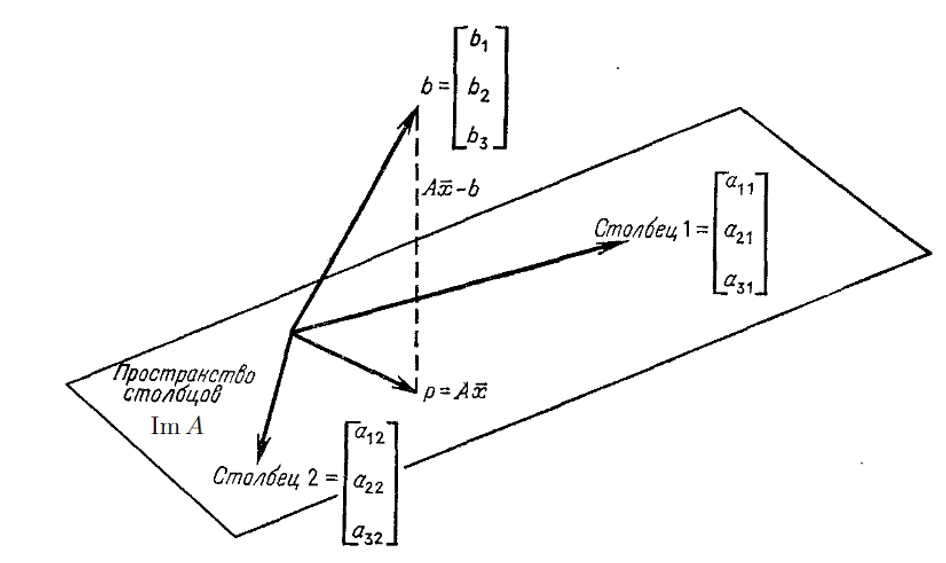
\includegraphics[width = 14 cm]{mnk.png}
\end{center}
Тогда $p = Pb$, где $P$ - матрица проектирования:
\[ P = A \cdot (A^T \cdot A)^{-1} A^T\]
Добавим, что невязка может выражаться, как $ b - p = b - Pb = b(E - P)$, и она ортогональна $\operatorname{Im} A$. Из этого факта и выводится знакомое нам уравнение метода наименьших квадратов. \\
Для любого нетривиального набора коэффициентов линейной комбинации столбцов матрицы $A$ (набор запишем в виде произвольного вектора $w$) справедливо, что их скалярное произведение с вектором невязки нулевое:
\[ (Aw)^T \cdot (A\bar{x} - b) = w^T \cdot (A^TA\bar{x} - A^Tb) = 0\]
Так как $w$ - произвольный ненулевой вектор, то именно второй множитель равен нулю. 
\begin{center}
   1. $Ax = p$ имеет \textit{единственное} решение
\end{center}
Эта ситуация хорошо изучена в стандартном МНК:
\[ A^TA \cdot x = A^T b \rightarrow \bar{x} = (A^T \cdot A)^{-1} A^T \cdot b\]
Единственная проблема систем из случая 1 в том, что $b$ не является точной линейной комбинацией исходных столбцов (например, из-за погрешностей в измерениях). Решив эту проблему, система становится 'обычной' и разрешимой. Для этого должно выполняться хотя бы одно из условий:
\begin{itemize}
    \item $rg(A) = n$, то есть ранг равен количеству столбцов (неизвестных). Тогда столбцы линейно независимы.
    \item $A^TA$ имеет обратную матрицу.  
\end{itemize}
\begin{center}
   2. $Ax = p$ имеет \textit{бесконечно много} решений
\end{center}
Из всех векторов, удовлетворяющих $Ax = p$ нужно выбрать единственный, который будет примерным решением системы $\bar{x}$. Логично положить (для минимизации ошибки), что $\bar{x}$ имеет минимальную длину из возможных. Как мы установили в предыдущем разделе, любое решение разглагается на проекции на $\operatorname{pr}_{\operatorname{Im} A^T} x = x_r$ и
$ \operatorname{pr}_{\operatorname{Ker} A} x = x_n$. Отметим, что компонента $x_r$ сама по себе является решением $Ax = A(x_r + x_n) = Ax_r = p$. \\
\\
Матрица $A^+$, которая задана условием $\bar{x} = A^+ b$, называется \textbf{псевдообратной}. 
Рассмотрим схему, аналогичную той, которая рассматривалась в предыдущем очерке:
\begin{center}
    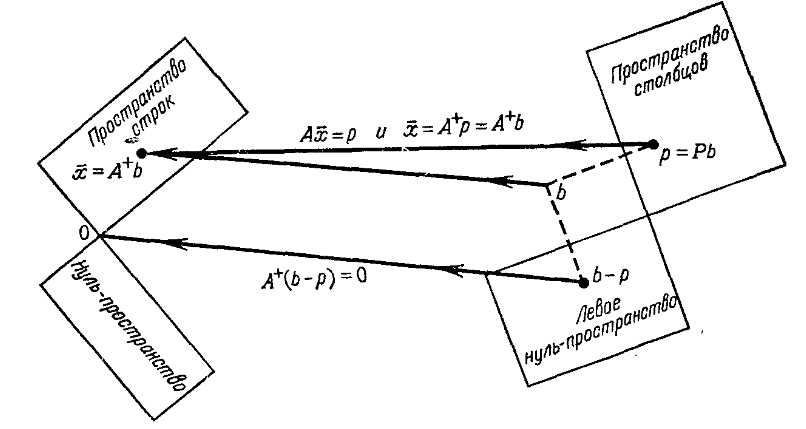
\includegraphics[width = 14 cm]{F.png}
\end{center}
Схема построена для исходной матрицы $A$, однако так как изучается обратная к ней, то стрелки идут уже в другую сторону. Теперь вектор $b$ разлагается на компоненты, а матрица $A^+$ проводит линейное преобразование. \\
Интересны частные случаи: \\
\\
$p = 0, b \perp Im A$, тогда $A^+$ переводит все векторы из $Ker A^T$ в нулевой. \\
$r = n, Ker A = {0}$. Поскольку пространство строк занимает теперь весь $\mathbb{R}^n$, то обращение можно однозначно задать. \\
Свойства псевдообратной матрицы:
\begin{itemize}
    \item $A^+$ имеет размер $n \times m$. 
    \item Например, из схемы видно, что $Im A = Im (A^+)^T$. Тогда $rg(A) = rg(A^+)$.
    \item $(A^+)^+ = A$
    \item $AA^+ = P$, так как $AA^+b = A\bar{x} = p = Pb$. 
\end{itemize}
Из последнего пункта можно вывести 'формулу' для псевдообратной матрицы, но только в том случае, когда $rg(A) = n$. Универсальная же формула выводится из сингулярного разложения. \\
\textbf{Пример}. Рассмотрим матрицы $A$ и псевдообратной к ней $A^+$. Процесс её вычисления пока оставим 'за кадром'.
\begin{equation*}
 \begin{cases}
&x- y + 2z =3,\\
&-x +2 y -3 z+u=6\\
&y-z+u=0 .\\
 \end{cases}
\end{equation*}
Матрица $A$: (как видим, $rg(A) = 2, r < n$)
\[ A = \begin{pmatrix} 
1 & -1 & 2 & 0 \\
-1 & 2 & -3 & 1 \\
0 & 1 & -1 & 1
\end{pmatrix} \]

Попробуем решить систему без знания о псевдообращении. Тогда нужно найти проекцию $b$ на пространство столбцов (выбираем линейно независимые первый и четвертые столбцы). Осуществляем обычную процедуру проектирования, считаем скалярные произведения, и получим, что $p = 0 \cdot e_1 + 3 \cdot e_4 = (0, 3, 3)^T$. \\
Решаем систему $A\bar{x} = p$ и получаем, что
\[\bar{x} = \begin{pmatrix} 3 \\ 3 \\ 0 \\ 0 \end{pmatrix} + C_1 
\begin{pmatrix} -1 \\ 1 \\ 1 \\ 0 \end{pmatrix} + C_2 \begin{pmatrix} -1 \\ -1 \\ 0 \\ 1 \end{pmatrix}\]
Можно показать, что наименьшая длина достигается при комбинации $C_1 = 0, C_2 = 2$. Тогда $\bar{x} = (1, 1, 0, 2)^T.$  \\
Псевдообратная выглядит так:
\[ A^+ = \frac{1}{9} \cdot \begin{pmatrix} 
3 & 0 & 3 \\
1 & 1 & 2  \\
2 & -1 & 1  \\
4 & 1 & 5
\end{pmatrix} \]
Матрица проекции $P = AA^+$:
\[ P = \frac{1}{3}\begin{pmatrix} 
2 & -1 & 1 \\
-1 & 2 & 1 \\
1 & 1 & 2 
\end{pmatrix} \]
Можно проверить, что проекция, рассчитаная вручную и вычисленная по формуле $p = Pb$, совпадут. Находим $\bar{x} = A^+b$ и получим $\bar{x} = (1, 1, 0, 2)^T$.

\end{document}